%\documentclass[letterpaper,11pt,preprint]{aastex}
\documentclass[11pt]{article}
\usepackage{graphics,graphicx}
\usepackage{natbib}
\usepackage{color}
\usepackage{times}
\citestyle{aas}
\usepackage{setspace}
\setlength{\bibsep}{0.0pt}

\setlength{\textwidth}{6.5in} \setlength{\textheight}{9in}
\setlength{\topmargin}{-0.0625in} \setlength{\oddsidemargin}{0in}
\setlength{\evensidemargin}{0in} \setlength{\headheight}{0in}
\setlength{\headsep}{0in} \setlength{\hoffset}{0in}
\setlength{\voffset}{0in}

% \makeatletter
% \newcommand{\mbe}{{\rm MBE}}
% \renewcommand{\section}{\@startsection%
% {section}{1}{0mm}{-\baselineskip}%
% {0.5\baselineskip}{\normalfont\Large\bfseries}}%
% \makeatother

% HCC's SPACE SAVING MAGIC FOR THE WINZ
\setlength{\parskip}{0.03in}
\setlength{\bibsep}{0.05in}

%\newcommand\mnras{\ref@jnl{MNRAS}}%
%\newcommand\nat{\ref@jnl{Nature}}
%\newcommand\apj{\ref@jnl{ApJ}}%
%\newcommand\jcap{\ref@jnl{J. Cosmology Astropart. Phys.}}%
%\newcommand\apjl{\ref@jnl{ApJ}}%
%\newcommand\procspie{\ref@jnl{Proc.~SPIE}}%
%\newcommand\aap{\ref@jnl{A\&A}}
%\newcommand\prd{\ref@jnl{Phys.~Rev.~D}}%
%\newcommand\aj{\ref@jnl{AJ}}%

\newcommand\mnras{{MNRAS}}%
\newcommand\nat{{Nature}}
\newcommand\apj{{ApJ}}%
\newcommand\jcap{{J. Cosmology Astropart. Phys.}}%
\newcommand\apjl{{ApJ}}%
\newcommand\procspie{{Proc.~SPIE}}%
\newcommand\aap{{A\&A}}
\newcommand\prd{{Phys.~Rev.~D}}%
\newcommand\aj{{AJ}}%



\makeatletter
\newcommand{\mbe}{{\rm MBE}}
\def\subsize{\@setsize\subsize{12pt}\xipt\@xipt}
\def\section{\@startsection {section}{1}{\z@}{1.0ex plus 
1ex minus .2ex}{.2ex plus .2ex}{\large\bf}}
\def\subsection{\@startsection {subsection}{2}{\z@}{.2ex 
plus 1ex} {.2ex plus .2ex}{\subsize\bf}}
\makeatother

%%%%%%%%%%%%%%%%%%%%%%%%%%%%%                                                                                                                                                                              
%%%%% Start of document %%%%%                                                                                                                                                                              
%%%%%%%%%%%%%%%%%%%%%%%%%%%%%                                                                                                                                                                              

%\usepackage{fontspec}
\usepackage{fancyhdr}
\pagestyle{fancy}
\headheight=12pt
\voffset -0.3in
\textheight=9.0in
\headsep=18pt
\lhead{McGill University}
%\chead{Sievers \& Chiang}
\rhead{Project \# 38558}
\renewcommand{\headrulewidth}{0pt}
%\renewcommand*{\bibfont}{\tiny}
%\usepackage{multicol}
%\usepackage{etoolbox}
%\patchcmd{\thebibliography}{\section*{\refname}}
%    {\begin{multicols}{2}[\section*{\refname}]}{}{}
%\patchcmd{\endthebibliography}{\endlist}{\endlist\end{multicols}}{}{}

\begin{document}

\begin{center}
{\bf A Deployable Signal Processing Engine for Radio Astronomy}
\end{center}
%\title{\bf A Deployable Signal Processing Engine for Radio Astronomy}
%\date{}
%\maketitle

%\setmainfont{Times}

%\pagestyle{plain}
\pagenumbering{gobble}
%\singlespace %xxx testing no aastex

%\section{Introduction}

%Building on the success of the Canadian Hydrogen Intensity Mapping
%Experiment (CHIME), we propose to build a new transportable back-end
%for next-generation radio telescopes that can be deployed to
%radio-quiet sites across the planet.  

% Traditionally, the back-ends were
%so expensive that it made sense to spend a lot of money on building
%large dishes and keeping the back-end fixed.  At its heart, the
%back-end is just a large computer, so Moore's law is having a dramatic
%impact on the traditional radio-telescope design.  This fact, plus switching to
%commodity parts, has lead to the back-end cost per incoming signal
%dropping by orders of magnitude.  In turn, for many science cases it
%no longer makes sense to build expensive traditional radio
%telescopes.  Instead, building very many cheap front-end elements
%coupled with a powerful back-end becomes a natural design.  

%{\setstretch{1.0}

As observational cosmologists, we are trying to understand some of the
most basic properties of the universe.  What is the nature of dark
energy?  Is the tension between different measurements of the Hubble
constant pointing to new fundamental physics?  When did the first
objects in the universe ignite, and what were they?  What did the
universe look like before these first stars formed, the so-called
``cosmic dark ages?''  Can we use fast radio bursts (FRBs) as a new
probe of cosmology?  In the last few years, radio astronomy has become
one of our most promising avenues for answering these questions.
Driven by Moore's law, the leading generation of radio arrays consists
of relatively inexpensive telescopes that require powerful
``back-end'' electronics to digitally process the vast quantities of
data. We propose to forge a new paradigm for radio astronomy by
building a sophisticated back-end electronics system---the McGill
back-end (\mbe)--- that is unique in that it is {\it portable} and can
thus service multiple telescope arrays in different locations.
Developing this portable readout technology will significantly reduce
the logistical overhead that is common to the remote observing
locations required for radio astronomy. Lowering this barrier will, in
turn, open large new swaths of discovery space.

The \mbe\ will handle the inputs from up to 1024 radio telescopes and
will process 3.25 terabits of data {\it{each second}}.  We will
leverage the successful technology developed at McGill for the
Canadian Hydrogen Intensity Mapping Experiment (CHIME;
\citet{Bandura16}), and, by many measures, the \mbe\ will be the
second largest of its kind in the world, surpassed only by CHIME
itself.  In the work covered by this proposal, we will build and
integrate the \mbe\ at McGill.  It will first be deployed, along with
a diesel rotary uninterruptible power supply (DRUPS) as part of the
Hydrogen Intensity and Real-time Analysis eXperiment (HIRAX;
\citet{Newburgh16}), the southern-hemisphere complement to CHIME.
Sievers and Chiang are co-PI and hardware lead, respectively, of the
international HIRAX collaboration, that is building and will use the
HIRAX telescope.  Along with our students and postdocs, we will use
HIRAX and the \mbe\ to answer fundamental questions about the
universe.  Concurrently, we will investigate sparsely populated areas
of northern Canada for promising sites for future \mbe\ deployments
after HIRAX (which will take 4-5 years to survey the southern sky),
answering new questions in cosmology.

\section{Research/Technology Development}

Hydrogen atoms naturally emit radio waves at a frequency of 1.4~GHz or
a wavelength of 21~cm.  As the universe expands, it stretches out
photons or ``redshifts'' them, driving them to lower frequencies.  As
a result, observing hydrogen at lower frequencies shows us the
universe when it was younger and more compact.  A radio telescope that
observes over a range of frequencies therefore, in a single
observation, naturally maps out the universe over a large fraction of
its life.  We can choose {\it{which}} periods of the universe's life
to study by selecting the corresponding frequencies.  Flexible
electronics like the \mbe\ can be used to study many different phases
in the evolution of the universe simply by switching the operating
frequencies.  The \mbe\ is transformational in that it gives us the
freedom to probe multiple pressing questions in cosmology in a way
that was not feasible in the past.  In this section, we will describe
the core science goals of the \mbe's first deployment at the heart of
HIRAX, followed by how modern radio telescopes work and the role the
\mbe\ fills.  Finally, we will describe how northern Canada's rare
combination of good infrastructure in sparsely populate areas makes it
a promising site for future \mbe\ deployments looking at the very
young universe.


\subsection{HIRAX and the \mbe\ as  Probes of Dark Energy}

When Albert Einstein worked out the equations of general relativity,
he saw that the simplest solution did not allow for a static
universe. Faced with this seeming unpleasantness, Einstein added a
term to his equations, called the cosmological constant, that he
thought would allow the universe to be infinitely old.  This term
arose from fixing the value of an integration constant to counter the
gravity from matter, and corresponds to giving a non-zero energy
density to empty space.  When presented with Edwin Hubble's evidence
for an expanding universe, Einstein dropped the cosmological constant,
calling it the ``biggest blunder'' of his life.  

There the matter stood for many decades, with the cosmological
constant being ignored.  From dimensional arguments, its natural value
is a Planck mass per Planck length cubed, or $\sim 10^{96}$
kilograms per cubic metre.  To get a sense of scale for just how huge
that density is, it corresponds to compressing all the matter in the
observable universe into a region the size of the nucleus of a single
atom.  Since the natural value is so large, it only made sense that
the cosmological constant be precisely zero.  However, as cosmologists
probed further and further into the universe, things began not quite
adding up.  In the 80's and 90's, studies of how distant galaxies
clumped together indicated that large-scale structures weren't growing
as expected in a universe with only matter in it ({\textit{e.g.}
  \citet{Park94}}).  Then in the late '90's, two separate groups
announced that distant supernovae were fainter than expected when
compared to nearby ones \citep{Riess98,Perlmutter99} in work that
would lead to the 2011 Nobel prize in physics.  Their data were
inconsistent with a matter-only universe, but agreed with a universe
in which expansion accelerated due to a cosmological constant.
Finally, as measurements of the cosmic microwave background (CMB)
transformed cosmology in the 2000's, we began to get percent-level
accuracy measurements of the vacuum energy contribution, with the
latest constraints from the Planck satellite indicating that today,
vacuum energy makes up $68.89\pm0.56$\% of the mass-energy in the
universe\footnote{while early CMB measurements needed an external
  measurement of the Hubble constant to make these statements, the
  improving measurements of the gravitational lensing of the CMB mean
  this is no longer true}\citep{Planck2018Params}.  As members of the
Atacama Cosmology Telescope (Sievers), South Pole Telescope (Chiang),
and Planck (Chiang) collaboration, the proposers have co-authored
dozens of papers over the last decade measuring the properties of the
universe and sharpening constraints on the vacuum energy.  

The disagreement between the natural ($10^{96}$ kg/m$^3$) and observed
(equivalent to about one atom per cubic metre) values of the vacuum
energy is ``probably the worst theoretical prediction in the history
of physics~\citep{Hobson06}!''  As such, there is no particularly good
reason to think that the simplest model, that of a cosmological
constant, is correct.  Cosmologists have packaged their ignorance by
calling the vacuum contribution ``dark energy,'' with the cosmological
constant but one of many possible models \citep{Ratra88,Steinhardt99}.
It {\textit{may}} turn out that a cosmological constant is a good
description, but it may well not.  If cosmologists were to find that
the vacuum energy changes with time, it would point to profoundly new
fundamental physics, radically reshaping our understanding of the very
nature of space and time.
%it would radically reshape our
%view of the universe and the very nature of space and time and point to profoundly new fundamental physics.
So far, the data we have in-hand are broadly consistent with constant
dark energy, within rather large errors.  However, it is of the utmost
importance to probe that by pushing to higher sensitivity and earlier
times in the universe, where different models for the time evolution
might be more apparent.  The need for improved dark energy constraints
over a broad range of time is particularly pressing because
values of the Hubble constant derived from low and high redshift data
now disagree at the 5$\sigma$ level.  If this discrepancy is found to
be real and not due to systematic errors, it could point to evolving
dark energy (see {\it{e.g.}} \citet{Freedman2017} and many others).
The tension has now even captured the popular
imagination\footnote{https://www.scientificamerican.com/article/have-we-mismeasured-the-universe/
  is one of several recent overviews}, heightening the urgency of
improved measurements.


%One way that dark energy is often
%parameterized is in terms of an {\textit{equation of state}}, where
%$w=\mathrm{P}/\rho$, where $\mathrm{P}$ is the pressure associated
%with dark energy, an $\rho$ is the energy density.  For a pure
%cosmological constant, $w=-1$.  A further generalization is to let $w$
%be a function of the size of the universe, $w(a)=w_0+(1-a)w_a$.  In
%this parameterization (others are possible), $a$ is the scale factor, the ratio of the size
%of the universe at a given point in time relative to the size today,
%and is the inverse of one plus the redshift $z$, $a=\frac{1}{1+z}$.  
%By definition, $a$ today is equal to one, and so measuring $w_0$ tells
%us about the modern day behaviour of dark energy, and $w_a$ tells us
%something about how that behaviour changes with time.  In these terms,
%the best current constraints are $w_0=-0.961 \pm 0.077$ while
%$w_a=-0.28^{+0.31}_{-0.27}$ \citep{Planck2018Params}.  So, while the
%evidence that dark energy behaves close to a cosmological constant
%today is moderately good, our limits on its evolution are very weak.
%This parameterization also has been used as a way of quickly comparing
%different experiments via the dark energy figure of merit (FoM), which
%is just one over the area of the 1-$\sigma$ contours in the $w_0,w_a$
%plane.  

Fortunately, nature has given us ways to map out the story of dark
energy, which affects how the universe has expanded as a
function of time.  The detection using supernovae relied on
the fact that astronomers understand their true brightness and
can use them as {\textit{standard candles}}.  With a standard candle,
by comparing the observed brightness of an object with its known true
luminosity, one can work out its distance.  Therefore, when supernovae
appeared fainter than their measured redshifts would have predicted,
dark energy was a natural explanation.  In addition to standard
candles, we can also use {\textit{standard rulers}}, a population of
objects whose intrinsic size is known.  By comparing the observed
angular size against the known true size, the distance to the object can
be deduced.  Nature has filled the universe with such standard
rulers, called baryon acoustic oscillations (BAOs).  

% BAOs arise from
%the first few hundred thousand years of the universe, when the density
%was nearly uniform everywhere and sound waves are the natural
%description.  The sound waves were driven by gravity and by pressure
%from free electrons dragging photons with them via Thomson
%scattering.  About 400,000 years after the big bang, the free
%electrons and protons very quickly combined to form neutral hydrogen
%atoms.  With no more free electrons, the sound waves stopped, and
%density perturbations began to grow simply via gravity, with their
%relative amplitudes frozen in.  We see these amplitudes today
%imprinted in the distribution of galaxies, with galaxy positions
%correlated on $\sim$500 million light-year scales today.  These ripples are
%called {\textit{baryon acoustic oscillations}} or BAOs.

BAOs arise from the same physics in the first 400,000 years after the
big bang that gives rise to the cosmic microwave background (CMB)
power spectrum.  Because the size scale of BAOs is set during the
young universe, and the CMB power spectrum is exquisitely well
measured \citep{PlanckSpectra2015,Louis2017,Henning2018}, cosmologists
understand very well how to tie the basic physics of the universe to
the BAO scale.  The BAO scale turns out to be large ($\sim$500 million
light years today), so their physics remains essentially linear, and
they simply scale with the size of the universe.  Therefore they
provide an almost ideal population of standard rulers. By observing
their angular size, we can map the history of dark energy.

The first detection of BAOs \citep{Eisenstein05} was made mapping
individual galaxies, but the very large scale of BAOs gives us another
tool, that of {\textit{intensity mapping}}.  Given the large size,
there can be hundreds of thousands of galaxies in any BAO volume, and
so one can take a very low-resolution image of the sky that averages
over large numbers of them.  The 21-cm hydrogen line is an especially
attractive tool for doing this.  Because hydrogen is the most abundant
element in the universe, the 21-cm line is relatively strong, and
unlikely to be confused by other radio spectral lines.  A radio
telescope that can map the sky at low resolution over a broad
frequency range can make a full 3-dimensional image of the BAOs, and
therefore trace out the history of dark energy.

HIRAX will be an array designed to measure the BAO spectrum over a
large area (up to 15,000 square degrees, or about 40\% of the sky) and
a large fraction of the history of the universe (from 2 to 6 billion
years after the big bang, or redshift from 2.5 to 0.8).  We need this
large volume and time range to measure enough BAO volumes that we have
good statistics, and to see how dark energy is affecting the growth of
the universe.  The hydrogen emission is faint ($100 \mu \mathrm{K}$),
so we need a very sensitive telescope.  However, because the signal is
on large (degree) scales, we do not need very high resolution.  These
facts set the HIRAX design of $\sim$ 1000 close-packed 6m-diameter
dishes.  The HIRAX collaboration will build the experiment in stages,
starting with a 128-dish pathfinder, followed by 256, 512, and finally a
full array of 1024 dishes.  Even with only 512 dishes, HIRAX will
provide improved constraints on the evolution of dark energy in
comparison to current measurements from all of cosmology (see Figure
\ref{fig:hirax_de}).  Measured by the dark energy task force figure of
merit\footnote{The figure of merit is defined relative to a model
  where the dark energy equation of state has a constant term $w_0$
  and and term that evolves with the size scale of the universe $w_a$
  where the size scale $a\equiv(1/1+z)$.}  (FoM), HIRAX-512 will have
an FoM value of 103, compared to the current state of the art of 95
(from CMB+BAO+supernovae, \citet{Planck2018Params}).  Crucially, HIRAX
is more sensitive at earlier times than current measurements, so if
the onset of dark energy domination occurred earlier than in the
standard cosmological model, HIRAX is uniquely positioned to observe
this effect.  The final 1024-element HIRAX array will have a projected
FoM of 285, which is comparable to or better than next-generation
surveys such as eBOSS in the 100-200 range \citep{Zhao2016}.

There are only a few BAO intensity mapping experiments worldwide
(MeerKLASS, \citet{Santos2017}; CHIME, \citet{Bandura16}; Tianlai,
\citet{Xu2015}; BINGO, \citet{Battye2013}).  Within this list, only
CHIME, HIRAX, and Tianlai are designed specifically to target early
dark energy.  HIRAX follows the groundbreaking work carried out by the
CHIME team, while being complementary and standing apart in several
important ways.  First, among these experiments, HIRAX is the
frontrunner in terms of collecting area, with 512 dishes improving
over CHIME by nearly a factor of two (and a factor of 3.5 with 1024
dishes).  HIRAX is also located in the southern hemisphere (CHIME and
Tianlai are both in the north), and independent measurements from both
hemispheres can be combined for improved precision on dark energy
constraints.  HIRAX's southern location also enables observations of
the Galactic center, which yields an advantage in searching for new
pulsars.  The HIRAX site is significantly more radio-quiet than the
CHIME site, and it will remain so as an area protected by the South
African government for radio astronomy research.  Finally, the
contrasting instrumental approaches between HIRAX and CHIME (dishes
versus cylinders, respectively) is absolutely essential for
cross-checking systematic errors and addressing the daunting task of
separating the minuscule cosmological signal from the emission from
our Milky Way galaxy, which is $\sim$1000 times brighter.

% This
%transformation has led to the a new model in which many inexpensive
%telescopes are piped into increasingly sophisticated digital%
%``back-ends'' that process vast amounts of data.  These back-ends are
%becoming increasingly flexible, capable of handling signal from a wide
%range of radio telescopes operating over wide ranges of frequency.
%This enables a new mode where the same back-end can be used with many
%different telescopes answering a wide range of basic questions about
%the universe.  However, practical considerations coupled with the
%questions being asked strongly influences the ideal sites to place
%radio telescopes.  Moore's law has now made it possible to make
%cutting-edge back-ends portable.  
%We propose to build a deployable
%back-end capable of processing 1,024 input streams with a combined
%data rate of 3.25 terabits per second.  Based on technology
%successully developed for the Canadian Hydrogen Intensity Maping
%Experiment (CHIME), its initial deployment will be to South Africa
%where it will form the heart of the southern analog to CHIME, the
%Hydrogen Intensity and Real-time Analysis eXperiment (HIRAX).  During
%HIRAX's four year observing run, we will search sites in northern
%Canada for sites free from human-generated interference, laying the
%groundwork for the next deployment.  Measured by the number of input
%streams processed together, this back-end will be the second largest
%in the world, second only to CHIME itself.

%\section{Research/Technology Development}%

%The Hydrogen Intensity and Real-time Analysis eXperiment
%\citep{Newburgh16} is a planned radio aray that will be sited in the 
%South African Karoo desert, on the future Square Kilometre Array (SKA)
%site.  HIRAX will consist of a large number of 6 metre diameter dishes
%(up to 1,024), in a compact layout.  Two of the central questions
%HIRAX will address are what is the nature of dark energy?  And what
%are fast radio bursts?  With its southern hemisphere location, HIRAX
%will also be perhaps the premier instrument for discovering new
%pulsars outside of the plane of the Milky Way.   Since the first
%deployment of the McGill back-end (\mbe) will be with HIRAX, we
%describe its science case first, followed by the essentials of how a
%radio telescope works and how the \mbe\ fits into HIRAX.  We then
%describe the current status and deployment plans for HIRAX, and
%discuss its complementarity it to CHIME.
%%the Canadian Hydrogen Intensity Mapping Experiment (CHIME).  

%\subsection{HIRAX as a Probe of Dark Energy}

%When Albert Einstein worked out the equations of general relativity,
%he saw that the simplest solution did not allow for a static
%universe. Faced with this seeming unpleasantness, Einstein added a
%term to his equations, called the cosmological constant, that he
%thought would allow the universe to be infinitely old.  This term
%arose from fixing the value of an integration constant to counter the
%gravity from matter, and corresponds to giving a non-zero energy
%density to empty space.  When presented with Edwin Hubble's evidence
%for an expanding universe, Einstein dropped the cosmological constant,
%calling it the ``biggest blunder'' of his life.  

%There the matter stood for many decades, with the cosmological
%constant being ignored.  From dimensional arguments, its natural value
%is a Planck mass per Planck length cubed, or about $5\times 10^{96}$
%kilograms per cubic metre.  To get a sense of scale for just how huge
%that density is, it corresponds to compressing all the matter in the
%observable universe into a region the size of the nucleus of a single
%atom.  Since the natural value is so large, it only made sense that
%the cosmological constant be precisely zero.  However, as cosmologists
%probed further and further into the universe, things began not quite
%adding up.  In the 80's and 90's, studies of how distant galaxies
%clumped together indicated that large-scale structures weren't growing
%as expected.  In a universe with only matter in it ({\textit{e.g.} \citet{Park94}}.  Then in 
%the late '90's, two separate groups announced that distant supernovae
%were fainter than expected when compared to nearby ones
%\citep{Riess98,Perlmutter99} in work that would lead to the 2011 Nobel 
%prize in physics.  Their data were inconsistent with a matter-only
%universe, but agreed with a universe in which expansion accelerated
%due to a cosmological constant.  Finally, as measurements of the
%cosmic microwave background (CMB) transformed cosmology in the 2000's,
%we began to get percent-level accuracy measurements of the vacuum
%energy contribution, with the latest constraints from the Planck
%satellite indicating that today, vacuum energy makes up
%$68.89\pm0.56$\% of the mass-energy in the universe\footnote{while
%  early CMB measurements needed an external measurement of the Hubble
%  constant to make these statements, the improving measurements of the
%  gravitational lensing of the CMB mean this is no longer
%  true}\citep{Planck2018Params}. 

%The disagreement between the natural ($10^{96}$ kg/m$^3$) and observed
%(equivalent to about one atom per cubic metre) values of the vacuum
%energy is ``probably the worst theoretical prediction in the history of physics! \citep{Hobson06}''
%  As such, there is no particularly
%good reason to think that the simplest model, that of a cosmological
%constant, is correct.  Cosmologists have packaged their ignorance by
%calling the vacuum contribution ``dark energy'', with the cosmological
%constant but one of many possible models \citep{Ratra88,Steinhardt99}.
%It {\textit{may}} turn out that a cosmological
%constant is a good description, but it may well not.  If cosmologists
%were to find that the vacuum energy changes with time, it would
%radically reshape our view of the universe.  So far, the data we have
%in-hand are consistent with constant dark energy within rather large
%errors, but it is of the utmost importance to probe that by pushing to
%higher sensitivity and earlier times in the universe, where time
%evolution might be more apparent.  One way that dark energy is often
%parameterized is in terms of an {\textit{equation of state}}, where
%$w=\mathrm{P}/\rho$, where $\mathrm{P}$ is the pressure associated
%with dark energy, an $\rho$ is the energy density.  For a pure
%cosmological constant, $w=-1$.  A further generalization is to let $w$
%be a function of the size of the universe, $w(a)=w_0+(1-a)w_a$.  In
%this parameterization (others are possible), $a$ is the scale factor, the ratio of the size
%of the universe at a given point in time relative to the size today,
%and is the inverse of one plus the redshift $z$, $a=\frac{1}{1+z}$.  
%By definition, $a$ today is equal to one, and so measuring $w_0$ tells
%us about the modern day behaviour of dark energy, and $w_a$ tells us
%something about how that behaviour changes with time.  In these terms,
%the best current constraints are $w_0=-0.961 \pm 0.077$ while
%$w_a=-0.28^{+0.31}_{-0.27}$ \citep{Planck2018Params}.  So, while the
%evidence that dark energy behaves close to a cosmological constant
%today is moderately good, our limits on its evolution are very weak.
%This parameterization also has been used as a way of quickly comparing
%different experiments via the dark energy figure of merit (FoM), which
%is just one over the area of the 1-$\sigma$ contours in the $w_0,w_a$
%plane.  

%Fortunately, nature has given us ways to map out the story of dark
%energy.  Dark energy affects how the universe has expanded as a
%function of time.  So, if we map that expansion out, we can work out
%the nature of dark energy.  The detection using supernovae relied on
%the fact that astronomers think they know their true brightness and
%can use them as {\textit{standard candles}}.  With a standard candle,
%by comparing the observed brightness of an object with its known true
%luminosity, one can work out its distance.  So, when supernovae
%appeared fainter than their measured redshfits would have predicted,
%dark energy was a natural explanation.  In addition to standard
%candles, we can also use {\textit{standard rulers}}, a population of
%things whos intrinsic size we know.  Then by comparing the observed
%angular size we see to the known true size, we can again work out a
%distance.  Nature has helpfully filled the universe with such standard
%rulers, called baryon acoustic oscillations (BAOs).  BAOs arise from
%the first few hundred thousand years of the universe, when the density
%was nearly uniform everywhere and sound waves are the natural
%description.  The sound waves were driven by gravity and by pressure
%from free electrons dragging photons with them via Thomson
%scattering.  About 400,000 years after the big bang, the free
%electrons and protons very quickly combined to form neutral hydrogen
%atoms.  With no more free electrons, the sound waves stopped, and
%density perturbations began to grow simply via gravity, with their
%relative amplitudes frozen in.  We see these amplitudes today
%imprinted in the distribution of galaxies, with galaxy positions
%correlated on $\sim$500 million light-year scales today.  These ripples are
%called {\textit{baryon acoustic oscillations}} or BAOs.

%Because the size scale of BAOs is set during the young universe,
%cosmologists understand very well how to tie the basic physics of the
%universe to the BAO scale.  Because the BAO scale is so large, their
%size just scales with the expansion of the universe.  Therefore they
%provide an almost ideal population of standard rulers - we know how
%big they are physically given how much the universe has expanded, and
%so by observing their angular size, we can map the history of dark
%energy.  

%The first detection of BAOs \citep{Eisenstein05}
%was made with galaxies, but the very large scale of BAOs gives us
%another tool, that of {\textit{intensity mapping}}.  Given the large
%size, there can be hundreds of thousands of galaxies in any BAO
%volume, and so one can take a very low-resolution image of the sky
%that averages over large numbers of them.  The hyperfine emission line
%of atomic hydrogen is an especially attractive tool for doing this.
%Hydrogen atoms in the universe radiate at a rest frequency of 1.4 GHz
%(or a wavelength of 21 cm) due to the energy difference between the
%proton and electron sping being aligned and anti-aligned.  Because
%hydrogen is the most abundant element in the universe, this makes the
%21 cm line relatively strong, and unlikely to be confused by other
%radio spectral lines.  So, by making a low-resolution map of hydrogen
%emission, we can trace out the BAOs.  Furthermore, because the
%expansion of the universe stretches out the 21cm photons, by observing
%at longer wavelengths, we can see the universe when it was younger.  A
%radio telescope that can map the sky with over a broad frequency range
%then can make a full 3-dimensional image of the BAOs, and therefore
%trace out the history of dark energy.  

%HIRAX will be an array designed to measure the BAO spectrum over a
%large area (up to 15,000 square degrees, or about 40\% of the sky) and
%a large fraction of the history of the universe (from 2 to 6 billion
%years after the big bang, or redshift from 2.5 to 0.8).  We need this
%large volume and time range to measure enough BAO volumes that we have
%good statistics, and to see how dark energy is affecting the growth of
%the universe.  The hydrogen emission is faint ($100 \mu
%\mathrm{K}$), so we need a very sensitive telescope.  The signal is on
%large (degree) scales, though, so we do not need a very high
%resolution telescope.  These facts set the HIRAX design of $\sim$ 1000
%close-packed 6m-diameter dishes.  We plan to build HIRAX in stages,
%first with 128 dishes, then 512, and finally a full array of 1,024
%dishes.  With 512 dishes, HIRAX constrains the evolution of dark
%energy comparable to current measurements from all of cosmology (see
%Figure \ref{fig:hirax_de}, and at 1,024 elements is comparable to
%next-generation experiments.  


\begin{figure}[t]
  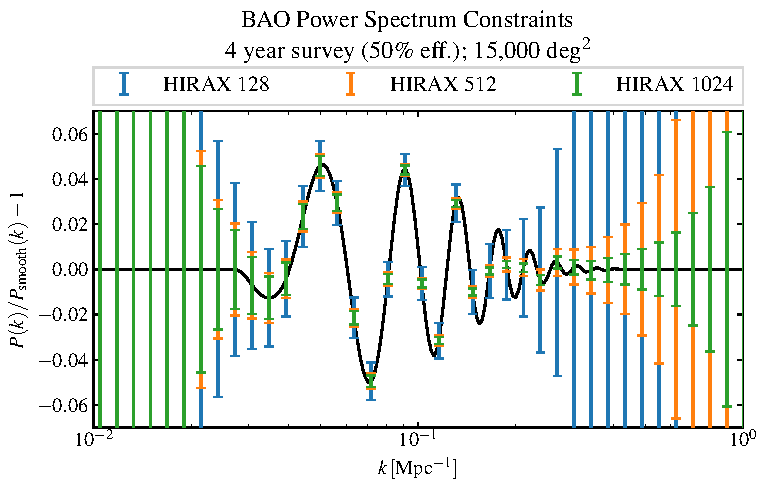
\includegraphics[height=2.5in]{hirax_bao_ps.pdf}
  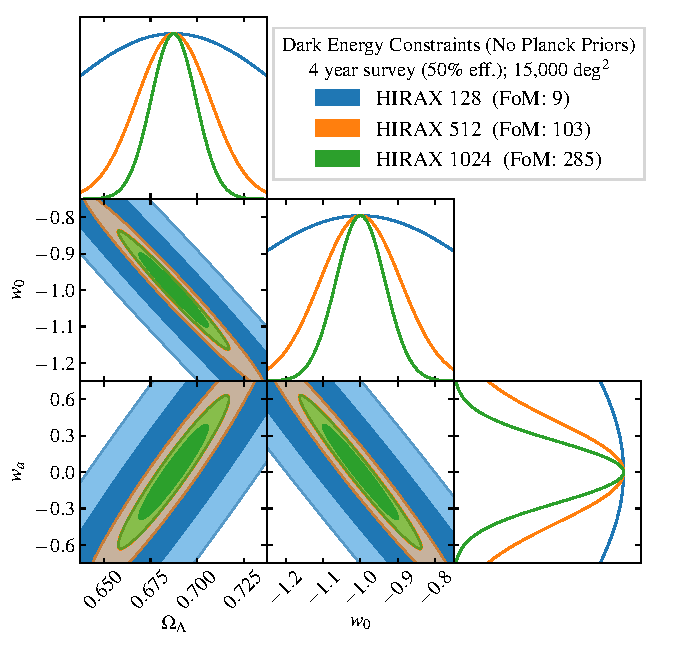
\includegraphics[height=2.5in]{hirax_de_constraints.pdf}
\caption{\small Left: HIRAX measurement of BAOs as a function of
  spatial wavenumber.  Blue/yellow/green are for four years of 50\%
  efficiency observations with 128/512/1024 dishes.  The size of the
  ripples decreases to the right, and the ripples are the periodic
  structure frozen in at recombination, when neutral hydrogen atoms
  formed.  Right: HIRAX constraints on dark energy cast in the
  $w_0,w_a$ plane.  With 512 dishes, HIRAX alone will improve on the
  current state of cosmology, which has a figure of merit of 95 (from
  CMB+BAO+supernovae, \citet{Planck2018Params}).  With the full 1024
  dishes, HIRAX will be comparable to next-generation dark energy
  surveys, which typically have figures of merit of $\sim 200$.
  \label{fig:hirax_de}
}
\end{figure}

\subsection{HIRAX and the \mbe\ as a Probes of Fast Radio Bursts}
Fast radio bursts (FRBs) are some of the most enigmatic objects in the
universe.  The first one was discovered by \citet{Lorimer07} in 2007,
just a decade ago.  As far as we know, they flash once, brightly, for
a thousandth of a second, and are generally never seen again (only
about 10 FRBs have been seen to repeat).  While we know virtually nothing about
what FRBs are, they seem arise from well outside the Milky
Way.  While theories abound, what truly gives rise to these flashes
bright enough to be seen from across the universe is a mystery.  While
we expect several thousand visible FRBs per day, the small fields of
view of current telescopes means that since their discovery, fewer
than 100 have been published, so their properties are not well
understood. Sievers' research has become increasingly focused on
FRBs, including how to find them \citep{Masui15}, possible origins of
FRBs \citep{Connor2016}, and how we can use them as a new probe of
cosmology \citep{Madhavacheril18,Walters2019}.

While HIRAX was designed to study dark energy, it is also a nearly
ideal instrument to find FRBs.  With 6m dishes operating between 400
and 800 MHz, the HIRAX field of view is $\sim 25-50$ square degrees.
The compact layout of HIRAX improves the efficiency of the FRB search
as well.  Modern algorithms have reduced by orders of magnitude the
computational load of searching a single beam for FRBs, to the point
that HIRAX will be able to search the $\sim$thousand beams that fill
its entire field of view.  Telescopes built for high resolution,
however, struggle to do this, and so they are likely to miss many
events.  HIRAX's high efficiency, along with the sensitivity from
having nearly 30,000 square metres of collecting area, means that we
expect to find nearly as many FRBs {\textit{every few days}} as have
been reported in total to-date.  While the rate in the HIRAX band is
still uncertain, with a rough value of 10-25 per day, CHIME has
recently reported FRB detections \citep{CHIME_ATEL,chime_frbs} ruling
out pessimistic estimates\footnote{CHIME has unofficially shown
  hundreds of detections, placing the event rate towards the
  optimistic side.  As of submission, however, these detections have not
  been published.}.

While a critical step to understanding what FRBs are is finding more,
an equally important step is to get accurate positions for them.  With
sufficiently accurate positions, extragalactic FRBs can be tied to a
host galaxy.  With a host galaxy, one can measure a redshift, and hence
a distance, to the FRB.  With a distance, one can finally infer an
energy scale for the bursts.  So far, despite extensive searches, only
a handful of FRBs have been seen to repeat.  Knowing where to look, astronomers
have pinpointed the location of the first repeating FRB to a dwarf
galaxy roughly 2.5 billion light years away ($z=0.19$).  Hundreds of
bursts have now been seen from that repeater, so we fundamentally do
not know if it is even typical of the FRB population.  Recently, the
first two non-repeating FRBs have been localized
\citep{Bannister2019,Ravi2019} and the host galaxy and absorption
properties are totally different from that of the localized repeater.
These detections have only served to deepend the mystery of FRBs.
 When coupled with outrigger stations the collaboration is building across southern
Africa (and for which funding has already been secured), HIRAX will
change the field.  With a total of several dozen inexpensive dishes at
a handful of sites working together with the core array powered by the
\mbe\ (see the next section for a technical description of how this
works), 
HIRAX will be able to determine the positions of a large
fraction of non-repeating FRBs to a thirtieth the size of typical
distant galaxies (0.03 arcsecond accuracy for 15$\sigma$
detections\footnote{The search space for FRBs is so vast that with
  perfectly Gaussian statistics, 9$\sigma$ fluctuations will be a
  regular occurrence.  Any non-idealities will drive that up, so
  15$\sigma$ is a conservative but realistic threshold for FRB
  detections.} in the core array).  
Not only will HIRAX plus
outriggers be able to localize thousands of FRBs, it will be able to
say from where within galaxies FRBs arise.  If FRBs are found to
originate near the cores of galaxies, their progenitors are likely to
be very different than if they arise from the outskirts.  With
localizations, we can even start to think using FRBs as probes of
cosmology, since they exquisitely measure the electron column density
along the line of site. This was first pointed out in
\citet{McQuinn2014}, who showed that just 100 FRBs with positions
(which HIRAX could find in a week) could be used to locate the
``missing baryons''.  They can also be used as probes of fundamental
physics, including placing limits on the photon mass
\citep{bonetti2017} and testing Einstein's equivalence principle
\citep{frb_equivalence}.  Sievers and collaborators have also shown
that FRBs can also be used to probe the kinetic Sunyaev-Zeldovich
effect, breaking the velocity-optical depth degeneracy in
next-generation CMB observations \citep{Madhavacheril18} and in
measuring the evolution of the gas fraction in the universe
\citep{Walters2019}.  

\subsection{Radio Telescopes and the \mbe}

An array of radio telescopes works by measuring the raw electric
fields from each individual telescope, and combining the signals from
every pair of telescopes.  This coherent combination of all the pairs
of telescopes lets the array work as a single whole, with
diffraction-limited resolution set not by the size of the individual
telescopes, but by the size of the array as a whole.  While individual
radio telescopes tend to have very poor resolution, arrays of radio
telescopes (often called interferometers) have given astronomers the
highest-resolution images ever taken.  For instance, the Event Horizon
Telescope, which combines telescopes across the planet to try to image
black holes, could resolve an orange on the moon\footnote{60
  micro-arcseconds resolution -
  https://eventhorizontelescope.org/building-larger-array}.

The way that interferometers combine the signals has a major impact on
the design, so we here lay out their basics.  First,
individual elements collect and amplify incoming radio waves.  These
elements might look like traditional radio telescopes, with large
parabolic reflectors (examples include JVLA, ALMA, MeerKAT, amongst
many others).  They might however consist of individual antennas
(PAPER, LWA), or multiple antennas hooked together with a first analog
combination stage (MWA, LOFAR), or even long cylinders with amplifiers
strung down the centre (CHIME, Ooty, UTMOST).  For modern digital
correlators, the next step is to digitally sample the electric fields,
and then use Fourier transform-based techniques to split the signals
into many narrow frequency channels.  At this point, all the frequency
channels from one antenna are together, but since we want to combine
all pairs of antennas together, we have to re-shuffle our data.  One
can think of the data as a 3-dimensional array, with time along one
axis, frequency along the second, and antenna number along the thirds.
This reshuffling, called the ``corner turn'' by radio astronomers,
amounts to take a matrix transpose in the frequency-antenna plane.
Once the data have been grouped by frequency, then every pair of
antennas are cross-correlated, which is mathematically equivalent to a
matrix multiply.  This design, where the data are split into frequency
channels, then cross-correlated, is called an FX correlator.  The part
that carries out the frequency splitting is usually referred to as the
F-engine, and the part that does the cross-correlation as the
X-engine.  The time-averaged cross correlation of a pair of antennas
(referred to as a baseline) is called a visibility, and is the
fundamental output of a radio interferometer.

While the individual steps in an FX correlator are conceptually
simple, the challenge is handling the truly immense amounts of data.
For the 512-dish version of HIRAX, we will have 1024 signals coming
into the \mbe, each with 400 MHz of bandwidth.  Using 4-bit
samples, that works out to over 3.2 terabits of data per second.  That
is nearly 20 times the data rate of the entire CANARIE network (2017
average), which services 157 Canadian higher education institutions
and over a million
users\footnote{https://www.canarie.ca/about-us/facts/}.  The
\mbe\ will take the incoming radio-frequency (RF) signals, digitally
sample them, split them into component channels, and carry out the
corner turn using custom backplanes.  It will then pass the
corner-turned data to a graphics processing unit (GPU)-based
correlator that will actually calculate the visibilities.  The
digitizing/sampling boards and custom backplanes were developed over
many years by Matt Dobbs' group at McGill, and successfully power CHIME.

While the raw data rate of the \mbe\ is far too high to store, one
case where it is directly relevant is in FRB localization.  To make
visibilities requires electric field-level data, so to localize FRBs
will require combining the electric fields from the outriggers with
those measured by the \mbe.  Continuously streaming electric field
data even from a small number of outriggers is prohibitive---for
instance, moving the raw data from an 8-dish station in Botswana would
exceed the entire country's international internet bandwidth.
Instead, the last 1-2 minutes of raw data from the \mbe\ will be
cached in RAM (probably by the GPU nodes in the X-engine).  When HIRAX
detects an FRB, the raw data will be saved to disk, and the outriggers
will be alerted that an FRB has gone off.  The outriggers will then
write their electric field cache to disk, and send just that bit of
data back.  The outrigger electric fields can then be combined with
the electric fields measured by the \mbe\ to localize FRBs.  By
themselves, the outriggers will not have enough sensitivity to find
FRBs, and HIRAX does not have the resolution to localize them, but by
working together, we will be able to localize non-repeating bursts.
Of course, the data rate from the \mbe\ is so huge that even saving
1-2 minutes of raw data requires 25,000-50,000 GB of RAM.

% Each crate
%with a custom backplane in the \mbe\ has 16 FPGA-based ICE boards
%(developed by Matt Dobbs' group at McGill).  Each board handles 16
%inputes, so a full crate works on 256 input RF streams.  The backplane
%in the crates carries out the corner turn for its 256 inputs, sending
%signals out over 10 gigabit ethernet cables.  For thousand
%element-scale arrays like HIRAX, Each GPU correlator node can take a
%10 Gb link from each \mbe\ crate, completing the corner turn, and the
%many terabits of data can be shuffled without the use of a single
%network switch.  

The \mbe\ will be housed in a custom-built, specialized shipping
container.  The container will be outfitted with multiple levels of RF
shielding, which is essential for protecting the radio telescopes from
contamination caused by spurious emission from the \mbe\ electronics.
The container will additionally be precisely temperature controlled in
order to maintain a safe and constant operating temperature for the
electronics and analog RF amplifiers.  All hardware will be installed,
integrated, and tested at McGill before being shipped to the HIRAX
site.  The highly modular nature also means that the \mbe\ can be
expanded simply by adding more crates as future funding permits.  The
GPU correlator will be housed separately.  Rapid developments in GPUs
mean that the cross-correlation part of back-ends have become obsolete
on short timescales.  For instance, NVidia has improved the on-paper
performance on 4-bit matrix multiplies, the core of what the GPUs do,
by a factor of $\sim$50 in about two years.  A single consumer-grade
board now has a theoretical performance of over 400 teraops for 4-bit
matrix multiplication.  In other words, the correlator one would
design today is radically different from the one CHIME deployed just
two years ago.  Conversely, the digitizing, channelizing, and
corner-turning operations that the \mbe\ will carry out evolve much
more slowly, and use much less power (1.5 kW per crate).  By
decoupling the F from the X part of the back-end, the \mbe\ will
remain a powerful tool for many years to come, and can be connected to
multiple telescopes and multiple GPU engines over its useful life.
This explains why the \mbe\ can be deployed to South Africa for HIRAX
for 4-5 years, and then redeployed to northern Canada with a new, by
then much-cheaper and lower power, GPU engine.  The \mbe\ will also
have flexibility in what frequencies it observes, and hence what
science it can pursue.  By selecting suitable (and inexpensive) analog
RF filters, the \mbe\ can observe {\textit{any}} 400 MHz frequency
chunk up to a maximum of 5 GHz.  With analog splitters, it can also be
configured to handle fewer telescopes over a broader frequency range,
{\textit{e.g.}} 512 inputs from 400 MHz to 1.2 GHz.

\subsection{HIRAX Deployment Plan and Status}

HIRAX will be one of the largest radio telescopes in the world.
Hence, we are planning a staged rollout.  In 2017, Chiang led the
construction of an 8-element prototype at the Hartebeesthoek Radio
Astronomy Observatory (HartRAO) outside of Johannesburg, South Africa.
The prototype has been invaluable in testing dishes and front end
components, and in gaining experience with back-end components.  The
8-element prototype and its first-light data are shown in Figure
\ref{fig:hirax8}.  It uses one of the same McGill-developed boards
that will go into the requested \mbe.  The South African Radio
Astronomy Observatory (SARAO) has agreed to host HIRAX on SARAO-owned
land about 15 km from the core MeerKAT site (30.6885S,21.5689E), where
the radio-frequency interference (RFI) environment is excellent in the
HIRAX 400--800~MHz band (see right panel of Figure
\ref{fig:hirax8}). The site agreement between SARAO and HIRAX is in
place as of August 2018, and construction of the first 128-element
HIRAX pathfinder (HIRAX-128) is expected to commence in 2020.  With
128 elements, we can save all the raw visibility data from the array,
and finalize and verify the data calibration/compression
pipeline. After many months of observations with HIRAX-128, we will
start construction of a 256-element version followed by a 512-element
version.  HIRAX-512 will be an extremely powerful radio telescope in
its own right, with limits on dark energy comparable to our current
knowledge from all cosmological data combined.  The \mbe\ as proposed
will support the full HIRAX-512. After a year of observing with
HIRAX-512, funding permitting, we will begin on HIRAX-1024.  We will
survey the entire southern sky visible to HIRAX, which we expect will
take approximately four years.  As part of our site agreement, SARAO
will provide access to power and data connections for HIRAX at least
through the commencement of Square Kilometre Array (SKA) operations,
which will give HIRAX time to complete the four year survey.  The site
development and dish production have been fully funded for HIRAX-256,
and the X-engine for HIRAX-512.  As part of the HIRAX installation,
the University of KwaZulu-Natal will purchase and install a diesel
rotary uninterruptible power supply (DRUPS) sufficient to power the
full array.  At the completion of HIRAX operations, McGill will assume
ownership of the DRUPS, and it and the \mbe\ will return to Canada for
our next observing program (beyond the scope of this proposal).

% However, that power envelope will be
%needed by SKA itself when it begins operations.  HIRAX will have
%finished its survey of the southern sky by the start of SKA, at which
%point the \mbe\ and the DRUPS will return to Canada where we will have
%developed our next observing programme.


%30 41 18.73S 21 34 07.98 
\begin{figure}[t]
  %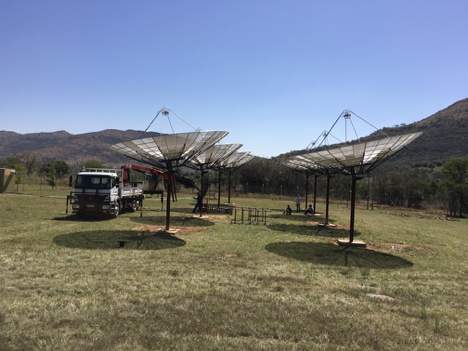
\includegraphics[height=1.4in]{hirax8.png}
  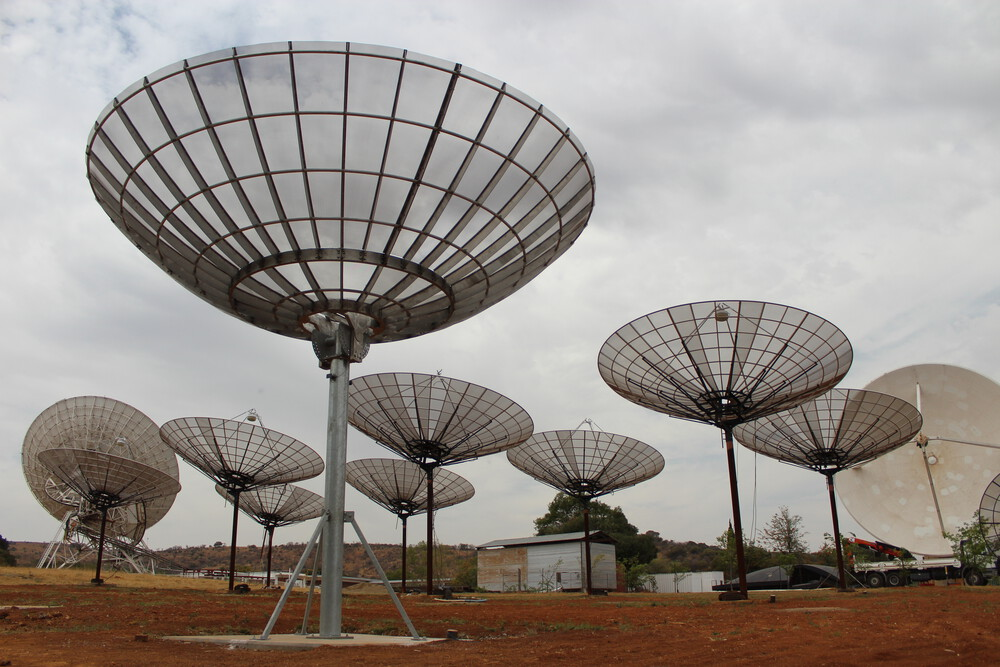
\includegraphics[height=1.4in]{rebcon_8element_small.jpg}
  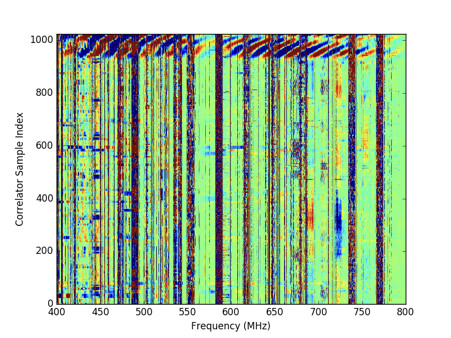
\includegraphics[height=1.6in]{first_fringe.jpg}
  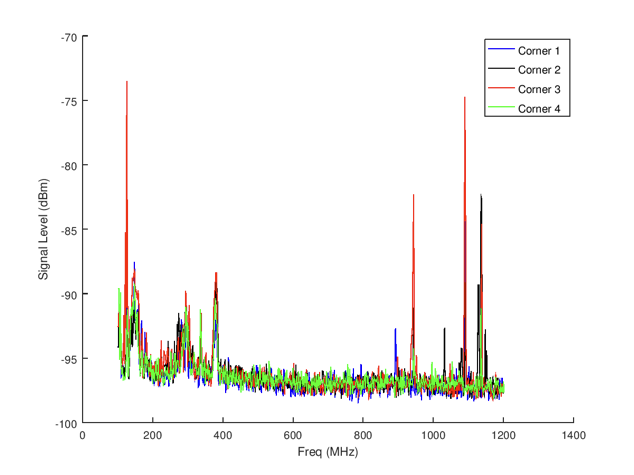
\includegraphics[height=1.6in]{hirax_site_rfi.png} 
\caption{\small Left: The foreground dish is custom-built laser-cut
  candidate dish for the final HIRAX design.  HIRAX 8-element prototype using off-the-shelf
  Chinese-manufactured 6m dishes is in the background.  The back-end uses the same boards
  that we will use for the \mbe.  Center:  The first-light data from
  the prototype.  The vertical stripes are human-generated
  interference (predominantly UHF TV stations). This interference
  would severely hamper HIRAX's ability to see BAOs.  The ripples at
  the top of the plot are the interference pattern from a bright
  source crossing through the field of view and show that the
  prototype is functioning end-to-end.  Right:  The RFI spectrum from
  the final HIRAX site on RFI-protected land owned by SARAO.  Unlike
  the prototype site, where at least half the data are lost to RFI,
  there is no visible RFI at the sensitivity level of the test
  equipment in the HIRAX science band.
  \label{fig:hirax8}
}
\end{figure}


%\begin{figure}[tbh]
%  \includegraphics[height=2.5in]{hirax_site_v2_marked.png}
%  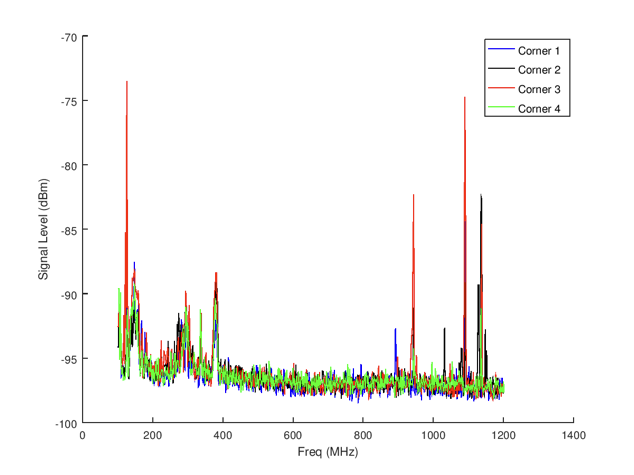
\includegraphics[height=2.5in]{hirax_site_rfi.png}
%\caption{\small Left: The location of the HIRAX site in the South
%  African Karoo desert.  The site is about 15 km away from the MeerKAT
%  core site, and 75 km from Carnarvon, the nearest town.  The site is
%  on RFI-protected land owned by SARAO.  Right: Daytime RFI spectra
%  measured from several locations on the HIRAX site.  At the
%  sensitivity of the test equipment, there is no detectable RFI in the
%  HIRAX 400-800 MHz band.  Cell phones are visible at 925-950 MHz,
%  military satellites appear in the 300 MHz range, and
%  intermittent RFI from airplanes is visible around 1.1 GHz.  Analog
%  filters will remove the out-of-band RFI at the telescope before
%  signals are sent to the back-end.
%  \label{fig:hirax_site}
%}
%\end{figure}

\begin{figure}[t]
  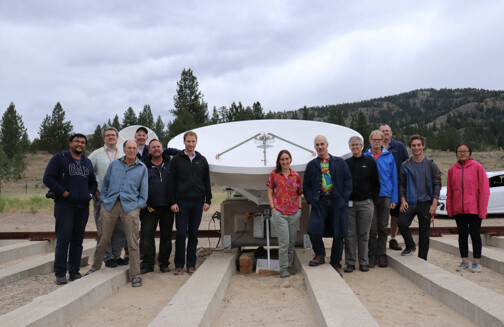
\includegraphics[height=2.1in]{d3a_team.jpg}
%  \includegraphics[height=2.5in]{rebcon_dish.png}
  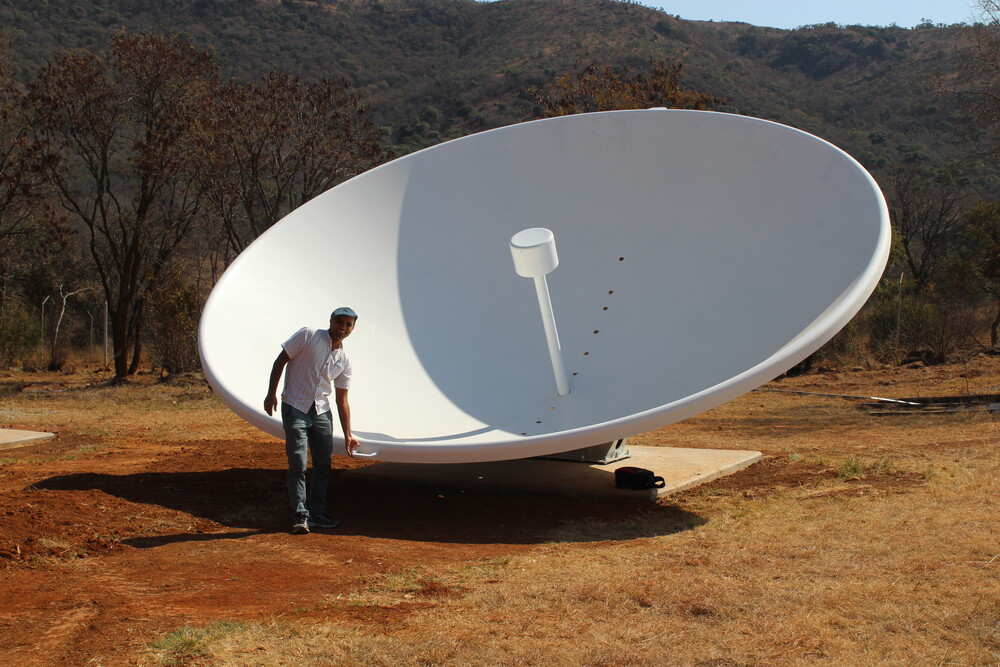
\includegraphics[height=2.1in]{mms_dish_kavi_small.jpg}
\caption{\small Left:  Canadian designed and built half-size composite
  HIRAX dish prototype installed at the Dominion Radio Astronomy
  Observatory.  The dish is fully instrumented and taking data..
  %For a few hundred dollar dish, the surface accuracy is outstanding,
  %with an RMS of 350$\mu$m.
  Right: Full-sized prototype HIRAX dish installed in South Africa.  This
  fiberglass dish is a candidate for the final design.
%Full-scale composite molds are currently being
%  manufactured in South Africa.  Right:  Full-sized metal prototype,
%  built in South Africa.  Surface accuracy and repeatability are still
%  being measured, but we expect them to meet HIRAX specifications.
  \label{fig:hirax_dishes}
}
\end{figure}

Much of the development work for HIRAX has been completed, with the
main challenge lying in the scaling to hundreds of dishes.  The
technology for the \mbe\ was developed for CHIME \citep{Bandura16},
and works in the field.  Similarly, the GPU correlator
\citep{Recnik15} works at scale and has been successfully proven by
CHIME, which recently published 13~new FRBs \citep{chime_frbs} and has
many other detections that are currently being analyzed.  Custom feeds
have been designed and built, and we continue to iterate to improve
their noise performance.
%  The signals from the telescopes will be sent
%via optical fiber to the back-end, in a procedure called radio
%frequency over fiber (RFoF).  Prototype RFoF transmit and receive
%boards have been demonstrated in the field at HartRAO, and the first
%production-scale order has been received and is undergoing testing.
%The main outstanding hardware development is the construction of the
%6m dishes.  
We have used low-cost ($\sim$800 USD) commercial off-the-shelf dishes
at HartRAO, but their optical design is not ideal for HIRAX (we
require dishes with a focal ratio of $f=0.25$, which shields the feeds
and reduces crosstalk between nearby antennas, key for a clean
cosmological measurement), and the manufacturing quality is rather
poor.  Consequently, we have been working with Canadian and South
African partners to develop suitable dishes.  One of the leading
options is a composite dish with a reflective metal mesh embedded in
fiberglass, and the design has been led by Gordon Lacy at the NRC.
Two half-scale prototypes have been constructed, and the measured
surface accuracy is 350$\mu$m RMS.  A full scale production-quality
mold has been fabricated in South Africa, with a measured surface RMS
of 800$\mu$m, less than 0.3\% of a wavelength.  A half-scale prototype
dish and the the first full-sized prototype made from the production
mold are shown in Figure \ref{fig:hirax_dishes}.
%  A second route is laser-cut
%metal dishes, with wire mesh attached to ribs. A full scale prototype
%has been completed, with a second ordered to compare repeatability.
%Samples of the dish prototypes are shown in Figure
%\ref{fig:hirax_dishes}.  We plan to verify the prototypes and make a
%final dish selection by the end of 2018.

HIRAX has already received a total commitment of 55,000,000 South
African Rand (about \$4,800,000 Canadian dollars, though exchange
rates are volatile) from the South African National Research
Foundation (NRF) and the University of KwaZulu-Natal for hardware
funding, along with significant funding (several million ZAR) for
graduate students and postdocs.  Additionally, Swiss collaborators
have secured 393,000 CHF (524,000 CAD) to build a GPU correlator that
will work in concert with the \mbe.  The current commitments, with the
availability of the \mbe, are enough to build and install at least 256
dishes.  The flexibility of the \mbe\ means that even at 256 dishes,
we can reconfigure the array to operate between 400~MHz and 1.2~GHz
simply by changing inexpensive analog filters upstream of the \mbe.
Even if funding for 512 dishes is delayed, \textit{we will fully
  utilize the MBE with funding already in place}.  We stress that
expanding the \mbe\ to handle HIRAX-1024 simply requires buying more
ICE board crates and installing them in the RF-shielded container.

\subsection{RF Lab and Antenna Development}

In order to integrate the \mbe\ and verify its performance, we propose
to establish a new radio instrumentation lab at McGill, led by Chiang.
This lab will house a comprehensive suite of test equipment that is
critical for troubleshooting \mbe\ subsystems and for demonstrating
successful end-to-end functionality.  The major required equipment
items include vector network analyzers (one 9-GHz benchtop unit to
span the full operational range of the ICE boards, and 6.5-GHz and
4-GHz portable units for field testing), a 3-GHz spectrum analyzer, a
6-GHz signal generator, 70-MHz oscilloscope, DC power supplies, LCR
meter, and precision 6.5-digit digital multimeter.

Because the redshifted hydrogen line is such a powerful and versatile
tool for cosmology, the new radio instrumentation lab will have
tremendous added value beyond the initial \mbe\ development and
deployment.  As just one example, in addition to enabling studies of
dark energy, the hydrogen line is also one of the most powerful
methods of probing the birth of the first stars.  A first detection of
this period of ``cosmic dawn'' was recently reported by the EDGES
experiment~\citep{Bowman2018}; however, the observed absorption trough
at 78~MHz was about {\it twice} the expected ampliutde.  If confirmed
by other experiments, this excess signal could point to a major
missing piece in the story of the universe, including possible new
fundamental physics such as early dark matter-baryon
interactions~\citep{Barkana2018}.  Although we are not proposing for
multiple \mbe\ deployments at this time, the integrated \mbe\ coupled
with the new radio instrumentation lab will lay the groundwork for a
wide range of future work, including low-frequency observations of
cosmic dawn.

In parallel with \mbe\ integration, the radio instrumentation lab will
also support the development of novel, self-contained antenna stations
that will be deployed in the Canadian north.  One of the greatest
challenges assocated with low-frequency measurements is RFI, with FM
radio in particular blinding telescopes in most locations.  In order
to access frequencies associated with cosmic dawn and earlier, it is
crucial to have a radio-quiet observation site that is far from
civilization and sheltered from human-generated transmission.  With
its sparse population but well developed infrastructure, {\it northern
  Canada presents a unique geographic advantage for low-frequency
  work}.  Chiang has already led an initial site survey on Axel
Heiberg island in Nunavut, and the preliminary results suggest that
the RFI environment is outstanding, with no persistent contamination
in the FM band.  Sievers has begun surveying areas in northern
Qu\'ebec which look promising for frequencies above 400~MHz.  The
radio instrumentation lab supported by this proposal will enable the
development of low-frequency antenna stations that will be installed
in northern Canada, taking full advantage of the clean observing
conditions.  The lab will also enable continued surveying efforts to
identify other radio-quiet sites in Canada.
% We have already deployed small radio antennas to one of the most
% remote locations in the world, Marion Island~\citep{PRIZM}, which
% lies halfway between South Africa and Antarctica, 2000~km from the
% closest permanent inhabitants.

\section{Researchers}\label{s:researchers}

PI Sievers and Co-I Chiang are key leaders in the HIRAX team, and the
proposed \mbe\ infrastructure is a major contribution that fulfills
our commitment to HIRAX and is critical for the project's overall
success.  Sievers is the co-PI of HIRAX and will lead the integration
of the \mbe.  He additionally holds a Canada-150 Research Chair
(\$1M/year level) and will fund the highly qualified personnel
required to built, test, and deploy the \mbe\ from his C150 funds.
Sievers has an extensive track record in cosmology, having worked on
many major international experiments spanning multiple research areas
(cosmic microwave background observations with both interferometers
and bolometric cameras, galaxy clusters, parameter estimation from
gravitational waves, 21-cm observations), and has the depth of
technical expertise and leadership experience needed to see the
\mbe\ through to success.  Sievers is additionally an expert in data
analysis, and he is well positioned to train highly qualified
personnel to face the challenge of distilling meaningful scientific
results from the deluge of data that the \mbe\ will generate.  Sievers
has co-authored over 100 scientific publications, with over 11,000
citations and an $h$-index of 59 (Google Scholar).  One key relevant
contribution was developing new fast pipelines for searching for FRBs
designed for use with HIRAX.  He and collaborators tested the pipeline
on archival Green Bank Telescope (GBT) data, and in the process
discovered one of the first FRBs known \citep{Masui15}.  This FRB was
the first one discovered with the GBT and the first one seen at
CHIME/HIRAX frequencies.  Lower-frequency searches had not seen any
FRBs, and the GBT detection thus confirmed for the first time that
future FRB events would be visible to CHIME/HIRAX.  Careful analysis
was able to show, although indirectly, that this burst must have
originated from outside the Milky Way.  The FRB event was also the
first one observed with linear polarization, which showed that there
was magnetized plasma near the source of the FRB.

Co-I Chiang will be responsible for establishing the McGill radio
instrumentation lab where the \mbe\ development and testing will take
place, and she will also lead the design, construction, and fielding
of the new low-frequency antenna stations for identifying candidate
future observation sites in northern Canada.  Chiang has a long
history of building and deploying instruments, and her wide-ranging
experiences spanning ground-, balloon-, and satellite-based platforms
place her in an ideal position to lead the instrumentation development
efforts proposed here.  Chiang is currently the hardware lead for
HIRAX, and she has overseen the successful construction of the HartRAO
eight-element HIRAX prototype and the development of the new,
custom-designed HIRAX dishes.  She is additionally the instrument and
deployment lead for a low-frequency observing program being conducted
from Marion Island; this work is particularly challenging since the
site is extremely remote, and access to the island is available only
once per year, via ship, for a three-week window.  Even a single
missing or broken part (without a spare) can delay progress for a
year.  Chiang has also worked in Antarctica on three separate
experiments: BICEP and SPT from the South Pole, and the balloon-borne
SPIDER from the coastal McMurdo station.  She has worked on data
analysis for the Planck satellite as a member of the High Frequency
Instrument core team, and as a Planck Scientist, she was a member of
the team that won the Gruber Prize in cosmology for 2018.  She has
co-authored well over 160 scientific publications, with over 40,000
citations (NASA ADS) and an $h$-index of 82.

The broader HIRAX team has the strengths required for a successful
experiment, with participation from around 25 institutions around the
globe\footnote{Collaborating institutions available at
  https://www.acru.ukzn.ac.za/~hirax/index.php/team/}.  McGill
Professor Matt Dobbs has developed the FPGA boards that lie at the
heart of the \mbe\ and now supplies them to a number of experiments.
He is a HIRAX collaborator and will supply the expertise needed to
supply the hardware and firmware for the \mbe.  Other key Canadian
collaborators include Keith Vanderlinde (Toronto) who built the CHIME
GPU-engine, and Kendrick Smith (Perimeter Institute) who enhanced the
algorithms in \citet{Masui15} and developed the FRB search pipeline
successfully used by CHIME.
% HCC: need to remove Gordon as a ``HIRAX collaborator?''
% Gordon Lacy (NRC) has demonstrated success
% with half-scale prototype dishes using inexpensive materials, and
% shown the half-scale prototype surface accuracy is a third of a
% millimetre.
Tzu-Ching Chang (JPL) led the first successful intensity
mapping detection \citep{Chang10} and her group contains experts in
electromagnetic simulations modelling HIRAX hardware.  Jeff Peterson
(Carnegie-Melon) and Kevin Bandura (West Virginia University) have
long experience with radio-frequency components and lead the RF
development, and also worked on the first intensity mapping detection.
Laura Newburgh (Yale) brings a wealth of experience from work on
CHIME, and has played a major role in HIRAX deployments to-date.  Aris
Karastergiou (Oxford) will lead the pulsar search with HIRAX, and
Amanda Weltman (University of Cape Town) will interpret the dark
energy constraints that come from HIRAX.  Kavilan Moodley (UKZN) took
over as South African HIRAX PI after Sievers joined McGill, and
oversees coordination with SARAO and site preparations.  Together, we
have already fielded a working prototype, and team members have
expertise in all the key areas required to make HIRAX work.  With
significant funding in place for other HIRAX subsystems, and with
\mbe\ contingency backstopped by the C150 chair, the team has the
skill, experience, and resources to make the \mbe\ and HIRAX work, and
push our understanding of the universe forward.

\section{Infrastructure}
The \mbe\ is unique in that it will be the only truly mobile
world-class back-end.  With the quick pace of GPU developments, we
expect the \mbe\ will be paired with many different GPU engines at
many different sites carrying out many different projects over its
life.  The \mbe\ is a major component of HIRAX and is {\it essential}
for the operation of the experiment.  The innovative and portable
\mbe\ platform will make it a game-changing contribution to the radio
telescope search for dark energy and FRBs, and will strengthen
Canada's leading role in the international cosmology community.  By
number of input signals, the \mbe\ will be the second-largest F-engine
in the world, trailing only CHIME\footnote{the total number of signals
  coming from the ASKAP, the Australian SKA Pathfinder, is also
  larger, but they are split into several independent groups which are
  not processed together}.  HIRAX will begin site preparations in late
2019 with construction of the 128-element stage starting in early 2020
and a 256-element stage shortly afterwards, likely late 2020 or early
2021.  We plan to start construction of HIRAX-512 roughly one year
later.  While a full 512-element array is not yet funded, HIRAX has
secured funding for at least 256 dishes. The flexibility of the
\mbe\ truly shines here since it can be reconfigured to work on
\textit{any} 400 MHz interval, up to $\sim$5 GHz.  So, during the
256-element stage, the \mbe\ can be reconfigured to work from 400 MHz
to 1.2 GHz simply by changing inexpensive analog filters.  Crucially,
an array of radio telescopes able to use the full capacity of the
\mbe\ is fully funded.

Since the hardware will be essentially identical to the F-engine built
by Matt Dobbs for CHIME, we have a very good indication of its cost.
The ICE boards, digitizers, and custom backplanes, with development
kit (which can also be used as spares in case of field failures), will
cost \$1,081,037 (budget item 9).  The \mbe\ uses 64 ICE boards with
sub-groups of 16, so a total of 80 ICE boards will let us field the
\mbe\ while having the minimum 16 boards in the lab needed to
test new firmware without interrupting science operations.
%\$729,600 USD, at a conservative exchange rate of 0.7, with an
%effective tax rate of 5\%, plus the cost of racks/power supplies to
%run the \mbe, totals for \$1,112,000 CAD.  
The RF-shielded enclosure, air-conditioned shipping container, and
shipping to/from the South African HIRAX site will be \$125,708 CAD
(budget item 7).  The cost is dominated by the custom RF shielding
built into the container.  Without the RF shielding, HIRAX will be
blinded by radio emission from the \mbe, and would not be allowed to
operate in radio-protected sites where it would interfere with other
telescopes.  The container will be housed in a parking lot at McGill
while the \mbe\ is being installed and tested, before field
deployments.
% (includingtax on the Canadian-acquired components).  
%Fortunately, for equipment temporarily deployed to South Africa for
%research purposes, there are no South African duty or VAT charges.
%loaned to South African universities for research purposes that will
%not stay in the country, 
%charged on the \mbe.  
The power in South Africa from the mains is not
clean, with frequent voltage sags, and power losses.  To keep the \mbe\
(along with the rest of HIRAX) working, we will need a diesel rotary
uninterruptible power supply (DRUPS).  SARAO has investigated the
matter carefully, and found these to be the most cost-effective
solution given the quality of the electricity supply.  That cost
will be about \$387,697 CAD (budget item 10), with UKZN purchasing this as an in-kind
contribution and McGill to retain ownership at the completion of
HIRAX.  We note that the DRUPS is overpowered for just the needs of the
\mbe\, but future deployments will also need to power the radio
receivers and the X-engine, and so the full power of the DRUPS will be
used.  Future Canadian deployments of the \mbe\ will need some form of
uninterruptible power supply, and so our baseline plan is to bring the
DRUPS back to Canada with the \mbe.  However we will revisit this as
future plans take shape.

Specialized lab and field RF test equipment will be \$202,909 CAD
(budget item 2).  The test equipment will stay housed at McGill,
modulo portable units brought into the field for short tests.
%including tax, 
Specialized lab RF components including assortments of amplifiers,
filters, bias tees, FPGA boards etc. will be \$48,209 (budget item 4).
Based on experience building stand-alone antennas on Marion, the cost
for each site-testing antenna station will be roughly \$24,335 total,
consisting of a mini shipping container to move the equipment and
environmentally protect the electronics on site (\$1,931), batteries
to work off-grid (\$288), solar panels and RF-quiet charge controllers
(\$1,601), the antennas and associated RF hardware (\$7,548), and a
custom-built readout electronics enclosure that houses a ``SNAP'' FPGA
board to process the data, frequency synthesizer for clocking, and
hard drives (\$12,967).  With three stations, needed to test sites
long enough to truly understand their RFI environments, the total cost
will thus be \$73,006 (budget item 6).
%.  With exchange rate and tax, this works out to \$33,000
%CAD per station, and we intend to deploy 3 stations to test a variety
%of sites long enough to truly understand their RFI environment.  This
%gives a total budget of \$99,000 for the base stations.  
The total request, including tax and matching contributions, is then \$1,918,566
CAD.  Matching will come from vendors (RF equipment supplier Keysight
has agreed to CFI matching) and from South African contributions.  

Successful operation of the specialized equipment described above
requires highly skilled personnel.  As described in
\S\ref{s:researchers}, Chiang already has significant resources and
expertise for supporting \mbe\ development, and she has extensive
experience training students in building cutting-edge instrumentation.
The McGill physics department has an electronics engineering team that
has been working closely with Chiang, and this team will provide
critical support for maintaining equipment and performing repairs if
needed.  The engineering team will additionally be an invaluable
resource for teaching students basic technical skills.

\section{Institutional Commitment and Sustainability}

McGill University has made a significant and sustained commitment to
radio astronomy.  It has been a major part of the successful CFI
proposal that built CHIME, and led the CFI proposal that added the
capability to search CHIME data for fast radio bursts.  Without the
extensive previous commitments from McGill, supported through Qu\'ebec
and national funding, construction of the \mbe\ described here would
not be possible.  It would require years of research and development,
costing far more.
% More broadly, Canada's
%investment in CHIME is what has enable HIRAX, which relies on several
%key CHIME technologies.  
McGill has further invested in this area
through the hiring of Adrian Liu, a theorist working in low-frequency
radio astronomy.  Indeed, the institutional expertise in this area was
a major factor in attracting the proposers to McGill.

The South African Radio Astronomy Observatory has agreed to host the
core HIRAX site, including the \mbe.  As part of the site agreement,
SARAO has committed to providing access to power and data connections
for HIRAX.  The transmission line supplying power to HIRAX also
supplies the Square Kilometre Array (SKA) site, and is near capacity, so the SARAO commitment
to provide access to power is essential.  The University of
KwaZulu-Natal (UKZN) has committed to site preparations and
backstopping the power installation costs, which will include power
and data line extensions and a transformer in addition to the DRUPS.
UKZN has further agreed to pay the power bill for HIRAX, including the
\mbe, during operations in South Africa.  The funding already secured
for HIRAX is enough to build a 256-element array that will run through
the \mbe.

With no moving parts, the reliability of the \mbe\ will be quite high
as long as the power supply is clean (hence the need for the DRUPS).
For the HIRAX deployment covered here, the \mbe\ will have a single
role, simplifying operations.  We have run the ICE board in the HIRAX
prototype for many months without needing human intervention, other
than rebooting after power outages.  After integration and
commissioning, the \mbe\ should run in a similarly hands-off manner.
However, given the scale of the the infrastructure, we will use
operating funds for part of an engineer's time to monitor the \mbe,
and troubleshoot as-needed.  This will amount to \$32,000/year over
five years.  In the event of a board failure (known to
be very rare), lab boards can be swapped in until replacement boards
can be acquired.  As a holder of a Canada 150 chair, Sievers will
cover the personnel costs associated with building the \mbe, and any
unforeseen operational costs that may arise.

Chiang has already taken up the space at McGill for the radio lab.
The requested lab infrastructure has no special needs beyond basic
requirements like lab benches and power, and no renovations of the
current lab will be required.  The antenna systems to be developed are
easily portable and can be deployed from a pickup truck/large
SUV-class vehicle.  Costs associated with test antenna deployments in
road-accessible regions to identify promising future sites will be
modest, and Sievers will cover any further expenses required for these
test deployments from C150 funds.  Sievers has already led preliminary
testing along the Route de la Baie-James and the Route du Nord, and
early results are promising enough to merit further testing,
especially at frequencies above 400~MHz.  These road-accessible
regions of Qu\'ebec are natural candidates for future large-scale
deployments serviced by the \mbe.  The most RFI-sensitive science
cases may require truly remote locations in the far north, such as the
McGill Arctic Research Station (MARS).  Chiang has secured an NSERC
Discovery Grant and Northern Research Supplement that will support
operations from these remote sites, and she has already led the first
MARS site surveying expedition in July 2019.  The antenna systems that
are intended for remote operations are custom designed and built by
students and postdocs, with assistance from the electronics
engineering team in the McGill physics department.  The development,
maintenance, and deployment of these systems is therefore performed
entirely in-house.  Following remote installation, team members will
regularly service the instrumentation and retrieve data, and the
associated logistics will be supported by annual requests to the Polar
Continental Shelf Program (PCSP, which already supported the site
surveying operations in July 2019).

\section{Benefits to Canada}

The infrastructure requested in this proposal directly addresses
several priorities and recommendations in the Canadian 2010 Long Range
Plan (LRP) for astronomy~\citep{lrp}.  Dark energy is highlighted
numerous times in the executive summary, underscoring the extreme
importance of this topic in modern cosmology.  The \mbe\ will expand
CHIME-like coverage to nearly the full sky, while enabling future
SKA-type science.  Support for CHIME and SKA science are both
emphasized in the Canadian astronomy plan.  We stress that Canadian
team members, both at McGill and elsewhere, and at student, postdoc,
and faculty level, will have full access to all HIRAX data should the
\mbe\ be funded, thus maximizing the scientific return.
Recommendation~7 of the LRP panel ``reiterates the need for \ldots
experimental astrophysics laboratories for \ldots instrumentation and
technology development.''  The \mbe\ will be designed, built,
integrated, and tested at McGill.  While its first deployment will be
overseas, the installation of the \mbe\ will cement McGill's position
as a leading institution within HIRAX.  The construction of the radio
lab at McGill by Cynthia Chiang will further strengthen the Canadian
and Qu\'ebec radio astronomy profile.  In addition to the training of
HQP, most of the equipment for the lab will be acquired through
Canadian suppliers.  A significant fraction of the instrumentation
developed in the radio lab will require custom machining and
fabrication processes, thus fostering numerous synergistic
opportunities with local industry partners.  For example, the HIRAX
composite dish prototypes have already been designed, built,
characterized, and installed at NRC, and the mount hardware (steel
work and concrete foundations) was contracted out to local companies.
As part of the development efforts for the low-frequency antenna
stations, we have already begun working with several Qu\'ebec-based
fabrication companies specializing in laser cutting, sheet metal work,
and automation/controls, and we are in the early stages of identifying
companies that can deliver power solutions for remote antenna
installations (including green, carbon-neutral technologies).

% Canadian team members will have full access to the data, and
% will be expected to participate in all aspects of the data analysis
% and science outputs.  This includes members at student, postdoc, and
% faculty levels.

The LRP further states that ``Demonstrating and maintaining Canadian
sovereignty over its Arctic territory has become an important national
priority. One method of accomplishing this goal is through Arctic
research programs; a major initiative is now underway to exploit the
Canadian High Arctic for astronomical observations.''  The report
focuses on optical observations, but the infrastructure in this
proposal brings new added value by expanding the astronomy landscape
in northern Canada to include radio observations.  A major component
of this proposal is to build hardware to search for sites with very
low amounts of radio-frequency interference (RFI) for the next
deployment of the \mbe.  The ideal location for a large array is one
with access to power and internet, but far from population centers.
Northern Qu\'ebec is especially attractive for this due to the
infrastructure accompanying the region's extensive hydropower
generation.  Multiple fiber optic networks run north, operated by the
Eeyou Communications Network.  One line runs along the James Bay road
with several branches cutting west to service towns along the coast.
A second line runs to the east, passing near Nemaska.  This level of
infrastructure in some of the least densely populated areas of the
planet is a truly unique opportunity.  With the revolution in radio
astronomy enabled by infrastructure like the \mbe, the shift towards
inexpensive dishes means we can hire local labour to build and install
future arrays.  This model has already worked well in South Africa,
where roughly twenty workers with no previous experience have been
hired to build the Hydrogen Epoch of Reionization Array (HERA),
another radio array hosted by SARAO.

In addition to addressing national priorities, the proposed
infrastructure also aligns strongly with the Qu\'ebec Research and
Innovation Strategy (SQRI).  One of the top priorities of the SQRI is
analytics of massive datasets.  The \mbe\ will process over 50 {\it
  exabytes} of digital data during its first deployment.  This data
set will be averaged to a daily rate of $\sim$50 TB/day, or over 70~PB
during the life of HIRAX.  In order to manage this enormous amount of
data, our team will develop novel compression techniques without
compromising the fidelity of the cosmology results, as well as write
algorithms to search for unexpected signals.  Due to the massive
volume, compression for HIRAX will have to happen on-site; with
redundancy built into the array the compressed volume should be a few
hundred GB per day.  We will copy this data back to Canada where we
will analyze the full survey on Compute Canada/Calcul Qu\'ebec
machines.  Detailed instrument modelling and simulations are key to
the success of HIRAX and interpretation of the results; this software
development addresses the SQRI goal of ``modelling, simulation, and
games.''  The \mbe\ will additionally open new research paths in
artificial intelligence, another goal that is specifically highlighted
by the SQRI.  Artificial intelligence has already been used to make
significant progress in FRB searches, and this initial demonstration
represents only the beginning of the full power that artificial
intelligence techniques have to offer.  Sievers has begun
collaborating with Liam Connor to apply his machine learning
techniques \citep{Connor2018} to improve the FRB search pipeline for
HIRAX, making it sensitive to a wider variety of bursts. The above
data- and computation-related skills are becoming rapidly and
increasingly sought after in industry across the world.  HIRAX is a
highly effective vehicle for cultivating the development of these
skills, which are readily transferable to industry applications.
Building up Canada's overall expertise in these areas will promote our
country's leadership and visibility on the international stage.


\subsection{Highly Qualified Personnel}


The infrastructure that is supported by this proposal will provide a
unique and interdisciplinary training environment for HQP.  The HQP
will have opportunities to play key roles in the detailed design of
the \mbe, subsystem testing, end-to-end integration, fielding of the
\mbe, and design/construction of new radio telescope stations that
will be supported by the \mbe.  The range of work is diverse and will
encompass both science and engineering.  In order to achieve the above
research goals, HQP will will be trained in mechanical and
electromagnetic design, electronics design and operation, instrument
characterization techniques, system integration, field work and
observations, and data analysis.  This type of training, in addition
to experience in leadership and mentoring, is critical for the next
generation of young scientists to push fundamental research forward.
The skills listed above are highly transferable and sought after by
industry, and the proposed infrastructure will thus open a wide range
of career options for HQP to contribute the fruits of their training
to positive socioeconomic growth.  A highly trained workforce is one
of the primary deliverables from the mission driven innovation
supported by this proposal.  Since the MBE will be installed in
multiple locations, the proposed infrastructure will involve a strong
component of international collaboration.  Interactions between HQP in
multiple countries will foster the growth of a racially- and
gender-diverse cohort.  PI and co-PI Sievers and Chiang already have
an exceptionally strong track record in bringing together HQP from a
wide range of backgrounds.  Since starting as permanent faculty in
2013, they have trained a combined total of 26 HQP representing thirteen
different countries (Botswana, Brazil, Cameroon, Canada, Chile, DRC, Ethiopia, Ghana, India,
Kenya, South Africa, Turkey, USA), including several students
from historically disadvantaged backgrounds.  The acquisition of the
\mbe\ will enable continued training of HQP with each PI supervising
5-6 HQP on average during the duration of the project through direct
supervision, for a total of 20-30 HQP.  Many more HQP will train at
other institutions in Canada and across the world.
%Past and
%present HQP trained by Sievers and Chiang since 2013 include
%* 1 research associate: R. Monsalve \\
%* 7 postdocs: M. Aich, B. Saliwanchik, H. Heilgendorff, T. Voytek, K. Knowles, S. Muya-Kasanda, V. Singh \\
%* 5 PhDs: T. Gogo, H. Heilgendorff, D. Olcek, L. Philip, O. Sengate \\
%* 8 MScs: J. Allotey, N. Ghazi, A. Gumba, K. Kesebonye, B. Kushiator, M. Mdlalose, O. Sengate, A. Zungu \\
%* 10 BSc Hons: N. Ghazi, A. Gumba, M. Gumede, K. Kesebonye, T. Moso, S. Ngobese, O. Seremane, W. Roberson, A. Moola, M. Mngqibisa \\
%
%Repeated names in the above list indicate successful completion of
%degrees and continued progress in academic studies.  Career milestones
%listed below include permanent jobs, prize fellowships, and other
%notable achievements of HQP trained by either Sievers or Chiang.  \\
%* V. Singh: Permanent research faculty at the Physical Research
%Laboratory\\
%* A. Zungu: Lecturer position at Sol Plaatje University\\
%* R. Monsalve: Lead postdoc on EDGES, and passed on many other
%opportunities to work on \mbe-related work at McGill.\\
%* M. Aich: Research scientist post, UKZN\\
%* K. Knowles: Square Kilometre Arrray postdoctoral fellowship\\
%* H. Heilgendorff: Square Kilometre Array postdoctoral fellowship\\
%* B. Saliwanchik: postdoctral position at Yale\\
%* O. Sengate: will be first-ever Botswanan astronomy PhD\\
%* J. Allotey: Square Kilometre Array internship, followed by PhD studies at Bristol\\
%* Nearly all other students in the above list have continued on to the
%next stages of their postgraduate studies\\


%* In early 2018, six students applied for the Dunlap/UToronto
%  astronomical instrumentation summer school. Five were accepted,
%  demonstrating their excellence among international standards. The
 % students have also participated in numerous other conferences and
 % workshops.  [ANYTHING NOTEWORTHY TO MENTION HERE?]
%

%Publications involving HQP:%
%
%* L. Philip et al., ``Probing Radio Intensity at high-Z from Marion:%
% 2017 Instrument,'' submitted to JAI 2018. L. Philip is the lead
% author and is my PhD student.
%* M. Jones et al., ``The C-Band All-Sky Survey (C-BASS): design and
% capabilities'', MNRAS 480, 2018. My postdoc and former PhD student,
% H. Heilgendorff, played a key role in developing the data analysis
% methods.
%* L. Newburgh et al., ``HIRAX: A Probe of Dark Energy and Radio
% Transients'', Proc SPIE 9906, 2016. One postdoc and two students
% (B. Saliwanchik, A. Gumba, L. Ngwenya) made critical contributions
% to instrument construction.

%[POSSIBLY USEFUL TEXT COPIED BELOW, NEEDS MORE WORK]

%These opportunities include interactions with industrial partners that
%are involved with subsystem manufacturing for our projects. The HQP
%who we have trained have backgrounds including physics, astronomy,
%mathematics, and engineering, and this broad spectrum yields many
%fruitful interactions.




%be very clear about added value to Quebec
%make sure to have sustainability part
%can cut down on intro
%make clear that due to fiber constraints the back end needs to be next to the dishes
%make more clear who HIRAX collaboration is, and who ``we'' refers to, e.g. HIRAX, Cynthia and me, Canada in general
%be careful to be clear why we need this tool as a JELF, not as part of a collaboration.  Always come back to own research goals.
%make clear outriggers are not part of MBE.  ``everything is interconnected, but always come back to what 
%   we are going to do with infrastructure here.''
%be clear that timescale to get MBE working is same as timescale to get HIRAX big enough to be used.  
%   this should go in the need for infrastructure.  be clear that we are still looking, and that 
%   we can use MBE with the things we already have funded.  
%get an email from Jo-Ann.  say that we have secured space from parking at McGill for integration here.  Make sure to
%   mention that containers will be locked/secured.  MAKE SURE TO GET 
%email site letter to Nathalie/Ada.  need to discuss operation/maintenance.  make clear who is paying for what.  
%   add that power will be covered by South African side in sustainability.  
%radio lab for building antennas.  make clear that will be Cynthia's lab at McGill, equipment will stay here, and we need it to
%    develop the infrastructure.
%describe in researchers section to be clear that we personally have tools/skills to use equipment here.  
%    JELF needs to be clear exactly what the role in development, but also in exploitation.  
%    needs to be clearly seen that we have expertise to exploit.  Matt is essential collaborator that we need
%    to develop the use of tools for our own research programme.  ``build on expertise Matt has
%    to go to next step on data where we have the expertise to exploit the data.''
%explain HIRAX consortium more strongly.  But, make clear we can't continue our research without access
%    to this piece of equipment.  Benefits to Canada and Quebec should make clear that science focus observations
%    move strongly to Canada.  
%McGill have already built something around radio, e.g. CHIME pathfinder, CHIME, demonstrates institutional commitment, and we have
%    network of collaborators here in place.  Look at CHIME CFIs, Vicki has been on a third one.  We can make clear
%    that McGill has made a serious commitment to this stuff, and that we can build on what has been funded.
%    make very clear that HIRAX has been enabled by previous Canadian investments in CHIME, put in sustainability.
%Use 8% for tax rate.  
%Be more clear about what is included in DRUPS cost.  Power is operating and doesn't count as in-kind.  
%    cost to extend power line to DRUPS, data connection are CFI-countable in kind probably.  
%    write in infrastructure section that installation costs will be born by UKZN.  
%    add installation costs to make sure line item is large enough.  UKZN should be vendor so 
%    they show up as in-kind.  UKZN should keep track of any costs/invoices associated with installation.  
%UKZN Administration needs to co-sign eventually the matching letter.  Nathalie needs to go through funding, site operations, maintenance. 
%Ada will share blurbs, need to talk about operations and maintenance.  
%IOF - 30% of 40% CFI, so 12% of CFI, we get 2/3, so 8%= 160K to use over 5 year period.  Should go in text in sustainability.  
%do not call parts spare parts, make clear they are for lab testing.  ``ICE Board Starter Kit''
%    Letter from Matt is fine for quote.  
%Don't talk about second container since coming from elsewhere.  Don't use word ``container'' for GPUs.  
%Ada will share with us quebec strategy, so we can align.  


%\bibliographystyle{apj}
%\bibliographystyle{abbrv}
%\bibliographystyle{abbrvnat} - this was latest, JLS
\begin{small}
\bibliographystyle{mybstv2}
\bibliography{cfi_jelf_sievers}{}
\end{small}
%total - 1112+153+376+214+42+33*5
\end{document}
